\documentclass{beamer}
\usepackage{verbatim} % For using /begin{comment}; /end{comment}
\usepackage{multirow}
\usepackage{booktabs}
\usepackage{textpos}
\usepackage{graphicx}
\usepackage{lmodern} % Font style
\usepackage{ragged2e} % For using \justify

\setbeamertemplate{frametitle}[default][center]
\setbeamertemplate{itemize items}{$\circ$}

\addtobeamertemplate{block begin}{\vspace{-8pt}}{}

\setbeamerfont{frametitle}{series=\bfseries} % Frame titles should be bold

\definecolor{mygray}{rgb}{0.23,0.27,0.29}

\setbeamercolor{background canvas}{bg=white}
\setbeamercolor{normal text}{fg=black}
\setbeamercolor{frametitle}{bg=mygray,fg=white}
\setbeamercolor{framesubtitle}{fg=white}
\setbeamercolor{block title}{fg=black}
\setbeamercolor{enumerate item}{fg=black}
\setbeamercolor{itemize item}{fg=black}


\begin{document}

\begin{comment}
\begin{frame}{Abstract}
\justify{Coronal seismology involves the investigation of magnetohydrodynamic
(MHD) waves and oscillatory phenomena that arise in the solar corona.
Properties of the observed modes are largely dependent on their
environment, and therefore can be used to extract atmospheric
parameters that are otherwise difficult to observe.
The general theory behind MHD phenomena is investigated here, along with
the characteristics of different modes
and the information that can be extracted from them.
A few methods are applied to data from the \emph{Atmospheric Imaging
Assembly} (AIA) instrument on the \emph{Solar Dynamics Observatory} (SDO).}
\end{frame}
\end{comment}

%\begin{comment}
\begin{frame}{Background and Motivation}
    Observations of waves and oscillations in coronal structures, such as loops
    and prominances, can reveal properties of the corona that are otherwise
    difficult to measure directly. Such properites include magnetic field
    strength and density. Characterizing the corona is important for
    understanding the dynamics of events that produce these oscillations, such
    as flares and coronal mass ejections (CMEs).
\end{frame}
%\end{comment}
\begin{comment}
\begin{frame}{Magnetohydrodynamics (MHD)}
    \begin{block}{Equations of ideal MHD}
        \begin{list}{}
            \item \textcolor{black}{mass continuity equation}
                $\frac{\partial\rho}{\partial{t}} +
                \nabla\left(\rho\mathbf{V}\right) = 0 $
            \item \textcolor{black}{equation of motion}
                $\rho\frac{\textrm{d}\mathbf{V}}{\textrm{d}t} =
                -\nabla{P} - \frac{1}{\mu_{0}}\mathbf{B}\times\left(
                \nabla\times\mathbf{B}\right) $
            \item \textcolor{black}{energy equation}
                $\frac{\textrm{d}}{\textrm{d}t}
                \left(\frac{P}{\rho^{\gamma}}\right) = 0$
            \item \textcolor{black}{induction equation}
                $\frac{\partial\mathbf{B}}{\partial{t}} =
                \nabla\times\left(\mathbf{V}\times
                \mathbf{B}\right)$
        \end{list}
    \end{block}
\end{frame}%--------------------------------------------------------------%
\end{comment}

\begin{comment}
\begin{frame}{Magnetohydrodynamics (MHD)}
    \begin{columns}
        \column{0.45\textwidth}
        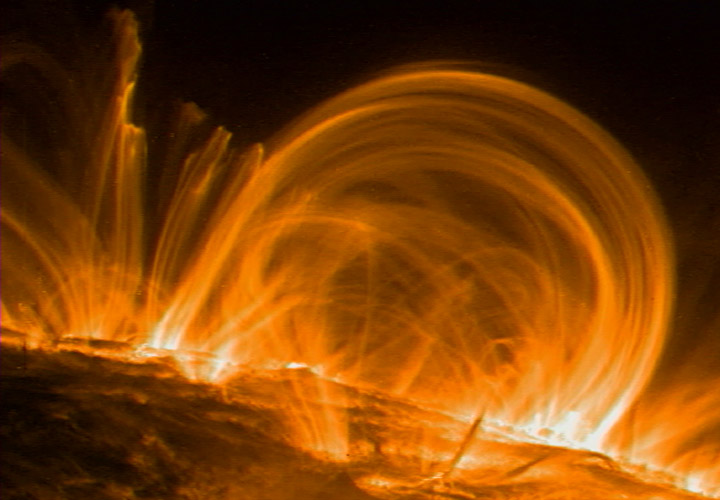
\includegraphics[width=\textwidth]{../loop.jpg}\\
        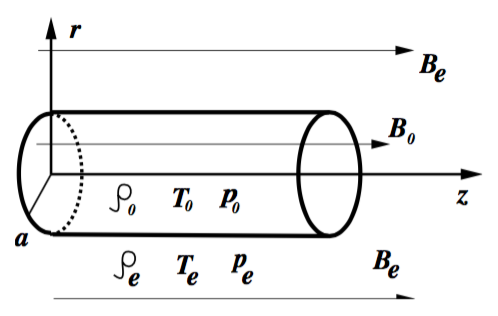
\includegraphics[width=\textwidth]{../cylinder.png}
        \column{0.55\textwidth}
        \begin{block}{Model}
            \begin{itemize}
                \item Straight cylindrical flux tube in uniform magnetic field.
                \item Equations of ``ideal'' MHD
                \item Characteristic wave speeds are determined by
                    $\rho$, $T$, $P$, and $\vec{B}$
            \end{itemize}
        \end{block}
        \begin{columns}[t]
            \column{0.4\textwidth}
            \begin{block}{\centering Sound speed}
                \begin{list}{}
                    \item $C_s$\hfill$\propto \sqrt{\cfrac{P}{\rho}}$\\
                        \vspace{0.5em}\hfill$\propto\sqrt{T}$
                \end{list}
            \end{block}
            \column{0.5\textwidth}
            \begin{block}{\centering Alfv\'en speed}
                \begin{list}{}
                    \item $V_A \propto \cfrac{B}{\sqrt{\rho}}$
                \end{list}
            \end{block}
        \end{columns}
    \end{columns}
\end{frame}%-------------------------------------------------------------%
\end{comment}

\begin{comment}
\begin{frame}{MHD modes in the solar corona}
    \begin{columns}
        \column{0.5\textwidth}
        \begin{block}{Main categories}
            \begin{itemize}
                \item Magnetoacoustic
                    %$C_s = \sqrt{\frac{\gamma P}{\rho}}$
                    \begin{itemize}
                        \item Fast %$k_{A_0} < C_{fast} < C_{A_e} $
                        \item Slow %$C_{T_0} < C_{slow} < C_{s_0} $
                    \end{itemize}
                \item Alfv\'en %$V_A = \frac{B}{\sqrt{\mu_0\rho}}$
            \end{itemize}
        \end{block}
        \begin{block}{Research Topics}
            \begin{enumerate}
                \item Kink oscillations
                \item Sausage oscillations
                \item Acoustic oscillations
                \item Propagating acoustic waves
                \item Propagating fast waves
                \item Torsional (Alfv\'en) modes
            \end{enumerate}
        \end{block}
        \column{0.55\textwidth}
        \begin{block}{}
        \begin{figure}
            \vspace{-2em}
            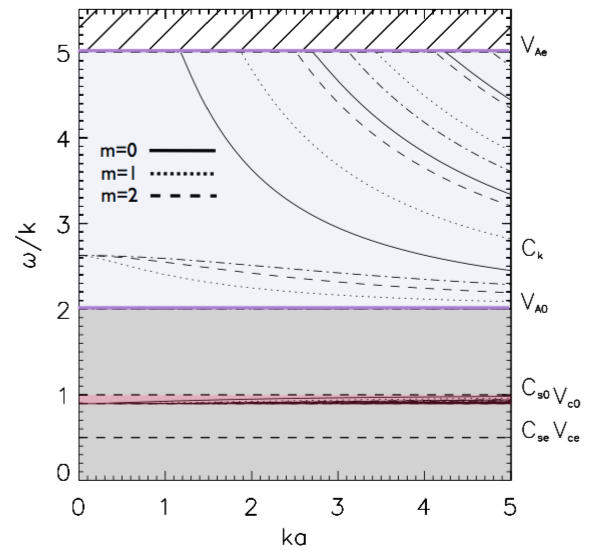
\includegraphics[width=\textwidth]{../disp_diagram.png}
        \end{figure}
        \begin{itemize}
            \item $ C_{k} = V_{A}\sqrt{\frac{2}{1+\rho_e/\rho_o}} $
            \item $ \xi(x) = \xi(r)e^{i(kz+m{\phi})} $
        \end{itemize}
    \end{block}
    \end{columns}
\end{frame}%-------------------------------------------------------------%
\end{comment}

\begin{comment}
\begin{frame}{Coronal seismology}{Technique and motivation}
    \begin{columns}
        %\column{0.5\paperwidth}
        \column{0.5\textwidth}
        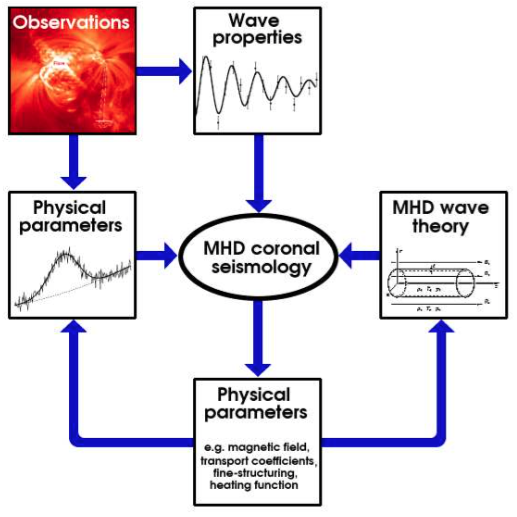
\includegraphics[width=\textwidth]{../schematic.png}
        %\column{0.5\paperwidth}
        \column{0.5\textwidth}
        \begin{block}{Elusive coronal properties}
            \begin{itemize}
                \item magnetic field strength, $\vec{B}$
                \item density, $\rho$
                \item Alfv\'en velocity, $V_A$
            \end{itemize}
        \end{block}
        \begin{block}{Motivation}
            \begin{itemize}
                \item Coronal heating
                \item Space weather prediction
            \end{itemize}
        \end{block}
        \begin{block}{Coronal seismology}
            \begin{enumerate}
                \item Observe disturbances
                \item Measure physical parameters
                \item Identify wave properties
                \item Extract physical parameters
            \end{enumerate}
        \end{block}
    \end{columns}
\end{frame}%-------------------------------------------------------------%
\end{comment}

\begin{comment}
\begin{frame}{Fast standing oscillations}{Kinks vs.\ Sausages}
    \begin{columns}
        \column{0.55\textwidth}
            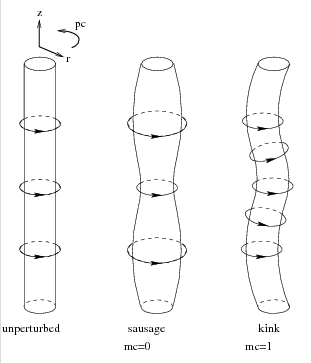
\includegraphics[width=\textwidth]{../kink_saus.png}
        \column{0.45\paperwidth}
        \vspace{-0.5in}
        \begin{block}{Period}
            \begin{itemize}
                \item $P=\frac{2\ell}{V_{ph}}$
                    ($\lambda=2\ell$)
            \end{itemize}
        \end{block}
        \begin{block}{Sausage}
            \begin{itemize}
                \item No loop spatial displacement
                \item Symmetric
                \item Intensity change\\ $\rightarrow$ density change
            \end{itemize}
        \end{block}
        \begin{block}{Kink}
            \begin{itemize}
                \item loop spatial displacement
                \item Asymmetric
                \item No intensity change
            \end{itemize}
        \end{block}
\end{columns}
\end{frame}%-------------------------------------------------------------%
\end{comment}

\begin{comment}
\begin{frame}{Standing oscillations vs.\ propagating waves}
    \begin{itemize}
        \item In loops, propagating waves damp before
            reaching opposite footpoint.
        \item Velocity and intensity are 90$^{\circ}$ out of phase
            for standing oscillations, and are in phase for propagating
            acoustic waves.
        \item Frequencies less than the cutoff are standing oscillations,
            waves with frequency greater than the cutoff propagate into
            the chromosphere.
    \end{itemize}
\end{frame}%-------------------------------------------------------------%
\end{comment}

\begin{comment}
\begin{frame}{Coronal loop oscillations observed with \emph{TRACE}}
    {Aschwanden et al. 1999}
    \begin{columns}
        \column{0.5\textwidth}
        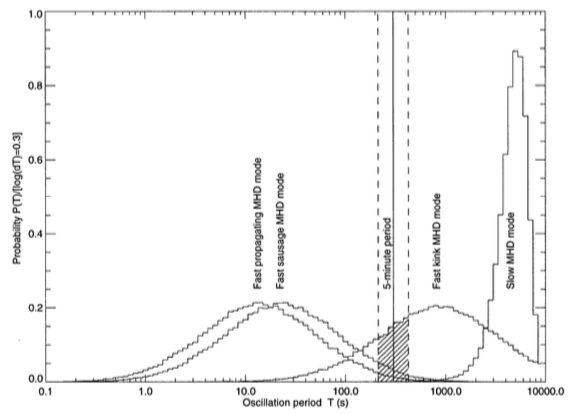
\includegraphics[width=\textwidth]{../kink7.png}
        \column{0.5\textwidth}
    \end{columns}
\end{frame}%-------------------------------------------------------------%
\end{comment}

\begin{comment}
\begin{frame}
    \vspace{0.25cm}
    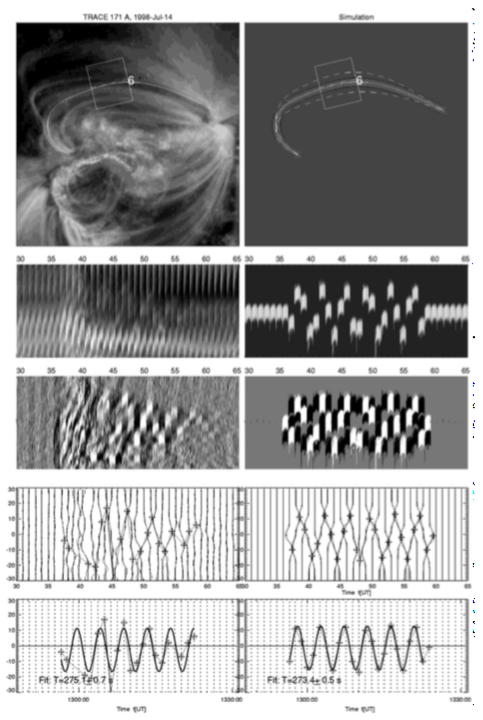
\includegraphics[height=\textheight]{../kink3.png}
\end{frame}%-------------------------------------------------------------%
\end{comment}
\begin{comment}
\begin{frame}{Excitation and damping of broadband kink waves in the solar
    corona}
\end{frame}%-------------------------------------------------------------%
\end{comment}
\begin{comment}
\begin{frame}[t]{``Observations of sausage modes in magnetic pores''}
    {Morton et al. 2011}
    \begin{block}{}
        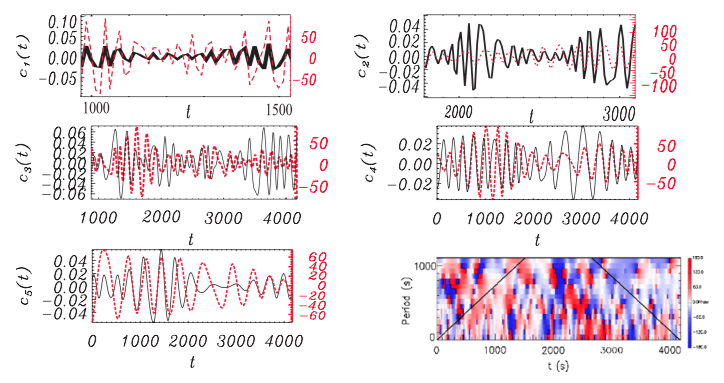
\includegraphics[width=\textwidth]{../saus2.png}
    \end{block}
    \begin{itemize}
        \item Periods $\sim$ 30{-}450 seconds (0.5{-}7.5 minutes)
        \item Possibly driven by 5-minute acoustic oscillations
    \end{itemize}
\end{frame}%-------------------------------------------------------------%
\end{comment}
\begin{comment}
\begin{frame}[t]{Alfv\'en waves}{Verwichte et al.}
    \begin{columns}
        \column{0.6\textwidth}
        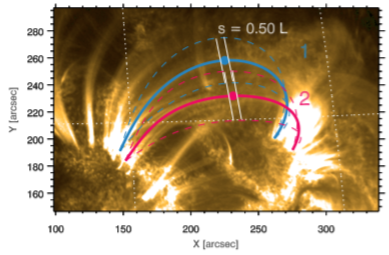
\includegraphics[width=\textwidth]{../tor22.png}
        \column{0.4\textwidth}
        \begin{block}{Objective}
            \begin{itemize}
                \item Determine Alfv\'en speed in two ways:
                    \begin{enumerate}
                        \item Coronal seismology
                        \item Magnetic extrapolation and spectral methods
                    \end{enumerate}
            \end{itemize}
        \end{block}
        \begin{block}{Observed}
            \begin{itemize}
                \item Two transversely oscillating loops triggered by flare
                \item AIA/SDO 171 \AA{}
            \end{itemize}
        \end{block}
    \end{columns}
\end{frame}%-------------------------------------------------------------%
\end{comment}
\begin{comment}
\begin{frame}[t]{Alfv\'en waves}{Verwichte et al.}
    \begin{block}{}
        \centering
        \vspace{-2em}
        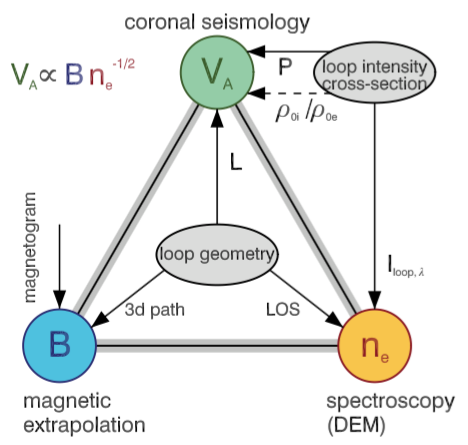
\includegraphics[width=0.6\textwidth]{../tor2.png}
    \end{block}
    ``The determination of the Alfv\'en speed from the observed phase
    speed lies at the heart of the seismological method\ldots''
\end{frame}%-------------------------------------------------------------%
\end{comment}

\begin{comment}
\begin{frame}[t]{Slow magnetoacoustic waves}{Robbrecht, et al. (2001)}
    \begin{block}{}
        %\column{0.5\textwidth}
        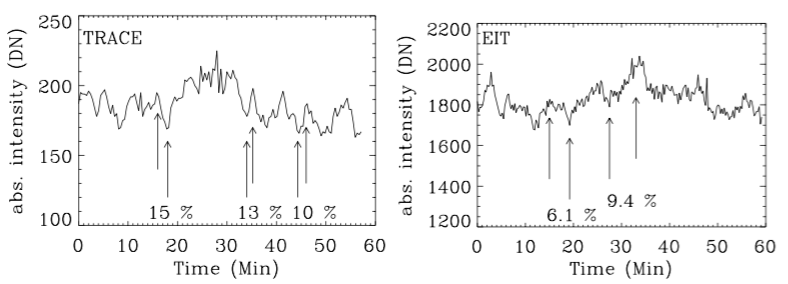
\includegraphics[width=\textwidth]{../pac1.png}
        %\column{0.5\textwidth}
    \end{block}
    \begin{block}{}
        \begin{itemize}
            \item Multi-wavelength observations
            \item Same wave, different speeds at different temperatures
            \item Loop contains sharp temperature gradient
        \end{itemize}
    \end{block}
\end{frame}%-------------------------------------------------------------%
\end{comment}
\begin{comment}
\begin{frame}{Important Properties}{From papers, reviews, etc.}
\begin{center}
    \begin{tabular}{c|c|c|c|}
        \cline{2-4} & {\textbf{\textcolor{black}{period}}} &
        {\textbf{\textcolor{black}{decay time}}} &
        {\textbf{\textcolor{black}{velocity}}}\\
        \hline \multicolumn{0}{|c|}{\textcolor{black}{kink osc}} &
            2{-}20 m & quickly & ---\\
        \hline \multicolumn{0}{|c|}{\textcolor{black}{sausage osc}} &
            30 s -- 7 m & --- & ---\\
        \hline \multicolumn{0}{|c|}{\textcolor{black}{acoustic osc}} &
            7{-}31 m & 5{-}30 m & 200 km s$^{-1}$\\
        \hline \multicolumn{0}{|c|}{\textcolor{black}{acoustic waves}} &
        140{-}420 s (2{-}7 m) & --- & 35{-}165 km s$^{-1}$\\
        \hline \multicolumn{0}{|c|}{\textcolor{black}{fast waves}} &
            --- & --- & $>$150 km s$^{-1}$\\
        \hline \multicolumn{0}{|c|}{\textcolor{black}{torsional modes}} &
            10 m & long & 1000 km s$^{-1}$\\
        \hline
    \end{tabular}
\end{center}
\end{frame}%-------------------------------------------------------------%
\end{comment}
\begin{comment}
{%
\setbeamercolor{background canvas}{bg=black}
\setbeamertemplate{background}{%
\parbox[c][\paperheight][c]{\paperwidth}{%
%\hspace{3cm}
\centering
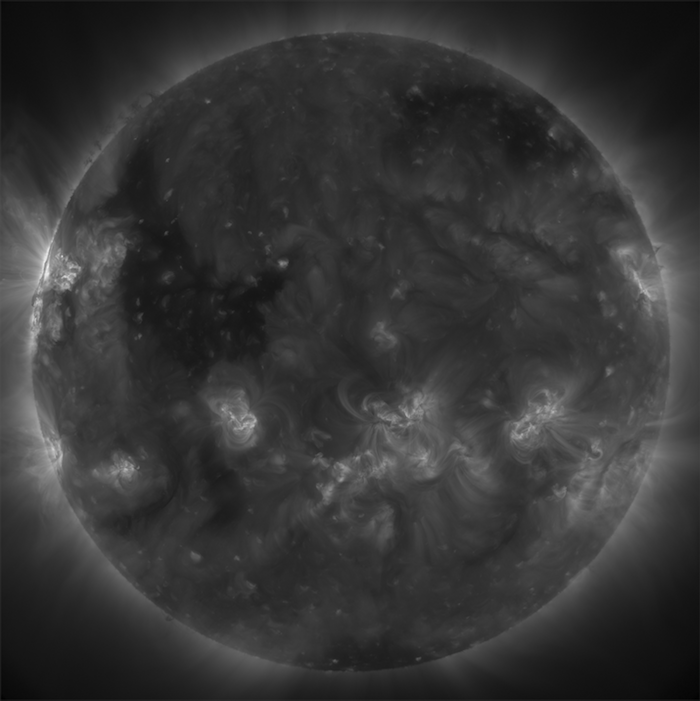
\includegraphics[height=\paperheight]{full_disk.png}}}
\begin{frame}[t]{Research}{AIA/\emph{SDO}}
    \hspace{-2em}Fe {\footnotesize XII, XXIV}\\
    \hspace{-2em}193 \AA{}\\
\end{frame}}%------------------------------------------------------------%
\end{comment}
\begin{comment}
\begin{frame}{Research}{Bright point (BP)}
    \begin{columns}
        \column{0.7\textwidth}
        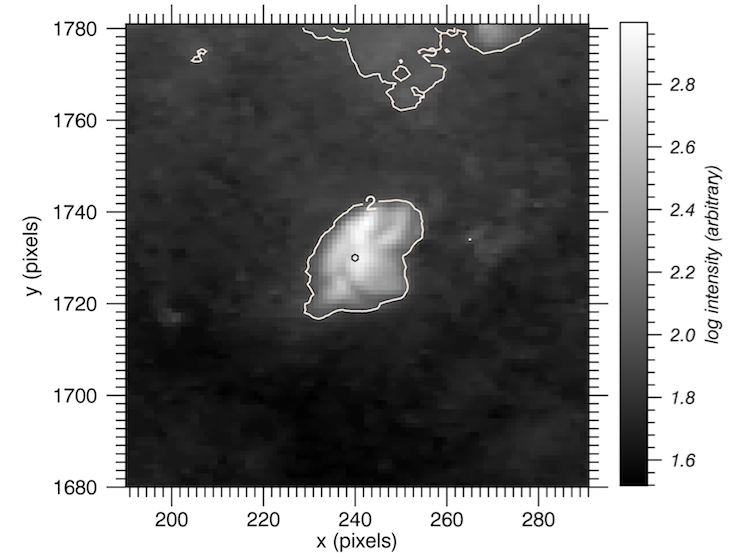
\includegraphics[width=\textwidth]{../figures/bp1_contour.png}
        \column{0.4\textwidth}
        \begin{itemize}
            \item Image:\\
                $\sim$ 45000 km across
            \item Bright point:\\
                $\sim$ 9000 km across
        \end{itemize}
    \end{columns}
\end{frame}%-------------------------------------------------------------%
\end{comment}
\begin{comment}
\begin{frame}{Research}{Plots}
    \begin{center}
        %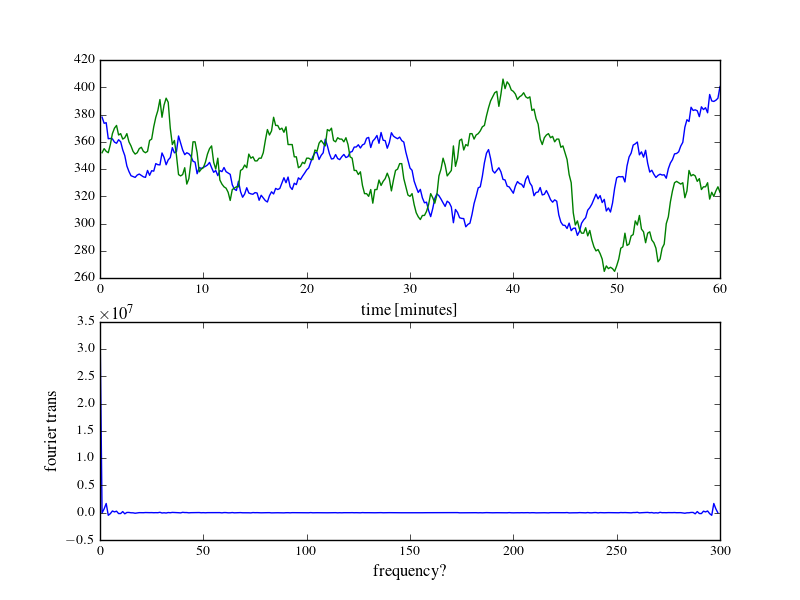
\includegraphics[width=0.8\paperwidth]{figure_1.png}
        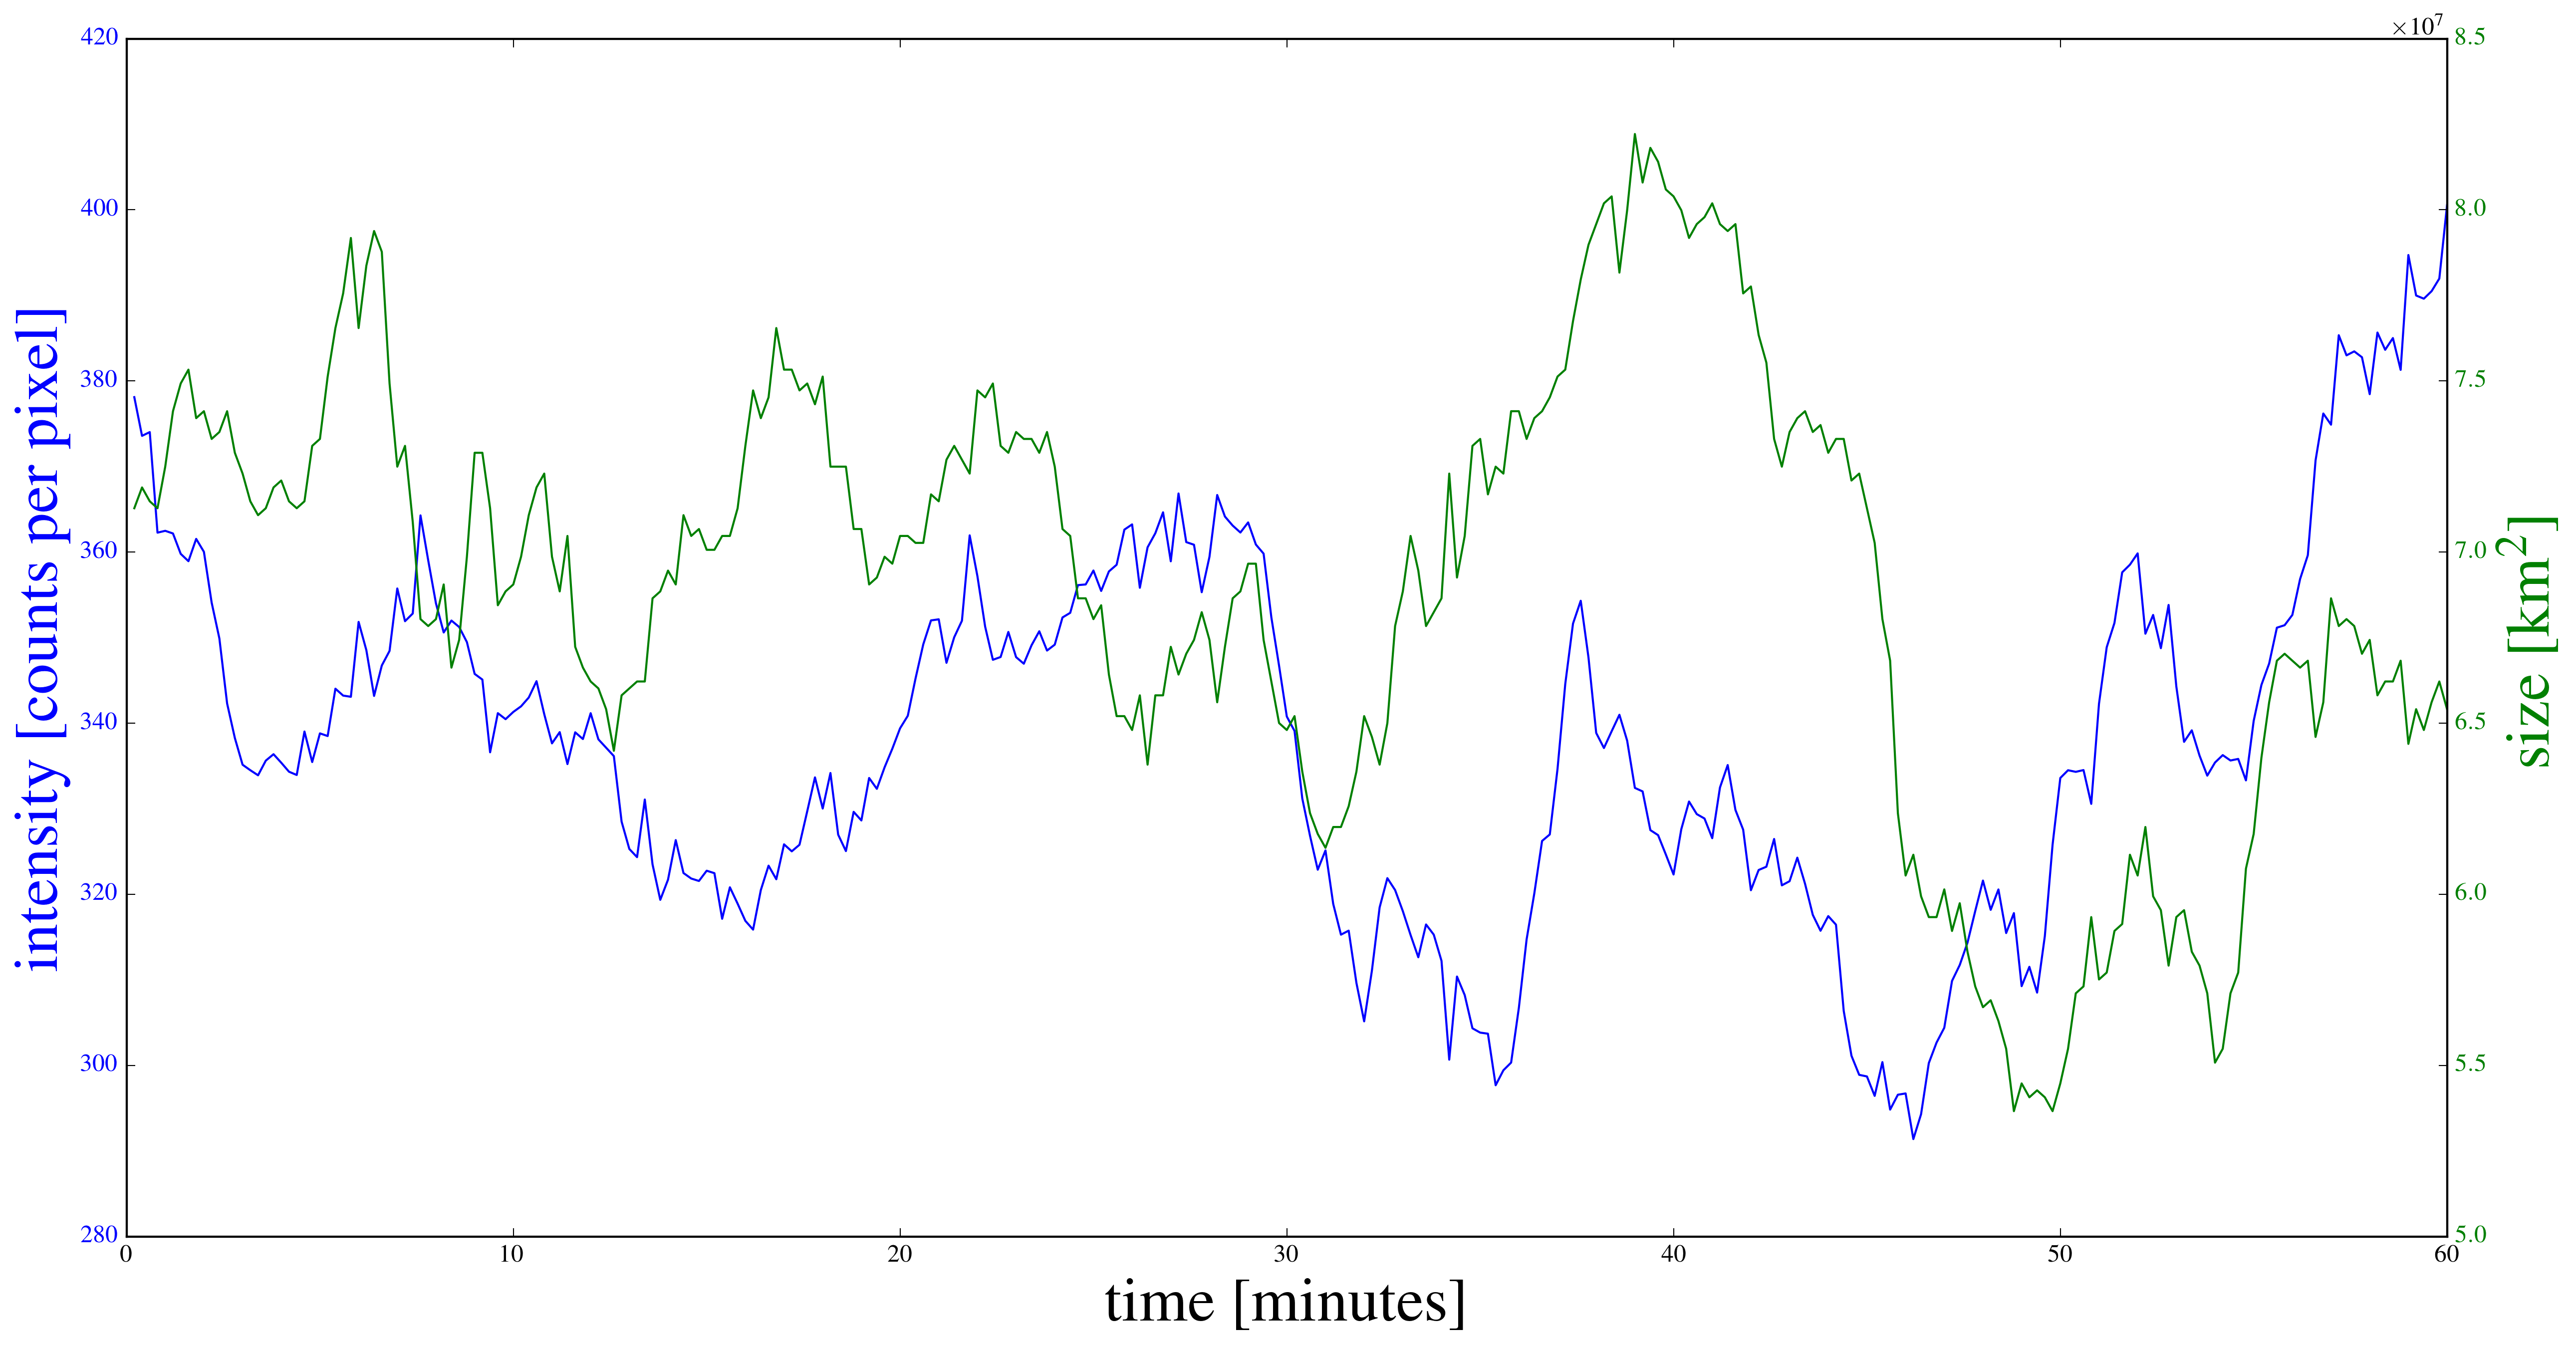
\includegraphics[width=0.8\paperwidth]{../plot2.png}
    \end{center}
\end{frame}%-------------------------------------------------------------%
\end{comment}

\begin{comment}
\begin{frame}{Research}{Cross-correlations}
    \begin{block}{}
        \begin{columns}
            \column{0.3\textwidth}
            \includegraphics[width=0.2\paperwidth]{../figures/bp1.png}
            \column{0.7\textwidth}
            \vspace{-2em}
            \includegraphics[width=\textwidth]{../cross.png}
            %\includegraphics[keepaspectratio=false,width=0.9\textwidth,height=1in]{cross.png}
        \end{columns}
    \end{block}
    \begin{block}{}
        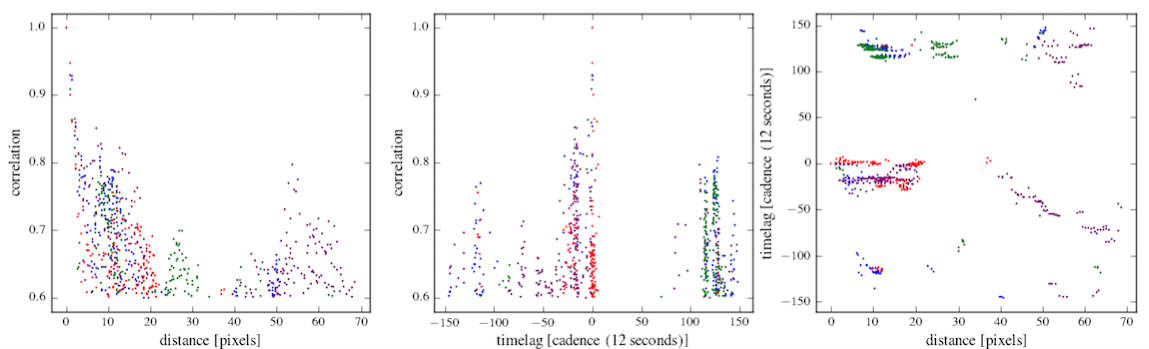
\includegraphics[width=\textwidth]{../test2.png}
    \end{block}
\end{frame}%-------------------------------------------------------------%
\begin{frame}[t]{Research}{Cross-correlation \& timelag images}
\vspace{0.25in}
    \begin{columns}
        \column{0.5\textwidth}
        \begin{block}{\centering Cross-correlation}
            \begin{center}
                \vspace{-0.25in}
                \includegraphics[height=0.5\textheight]{../figures/bp1_cc.png}
            \end{center}
        \end{block}
        \column{0.5\textwidth}
        \begin{block}{\centering Timelag}
            \begin{center}
                \vspace{-0.25in}
                \includegraphics[height=0.5\textheight]{../figures/bp1_tt2.png}
            \end{center}
        \end{block}
    \end{columns}
    \begin{center}
        2 pixels $\sim$ 1 arcsec $\sim$ 700 km
    \end{center}
\end{frame}%-------------------------------------------------------------%
\begin{frame}{Other questions and future work}
    \begin{block}{Other questions}
        \begin{itemize}
            \item What is the excitation mechanism for the observed
                disturbances?
            \item How are they damped, and what determines the timescales?
        \end{itemize}
    \end{block}
    \begin{block}{My future work}
        \begin{itemize}
            \item Download data in other wavelengths (i.e.\ coronal heights).
            \item Download data from other instruments,
                e.g.\ the Extreme Ultraviolet Variability Experiment
                (EVE) on SDO\@.
            \item Characterize other bright points in coronal hole,
                quiet sun, and active regions.
        \end{itemize}
    \end{block}
\end{frame}%-------------------------------------------------------------%


\begin{frame}{Coronal Seismology}
\end{frame}
\begin{frame}{Data}
\end{frame}
\begin{frame}{Cross-correlation results}
\end{frame}
\begin{frame}{Lightcurve results}
\end{frame}
\begin{frame}{Conclusions}
\end{frame}
\begin{frame}{Future Work}
\end{frame}
\begin{frame}{Acknowledgements}
\end{frame}
\end{comment}
\end{document}
